% !TeX encoding = UTF-8
\documentclass{protokol}

\usepackage{pdfpages}
\usepackage{tikz}
\usetikzlibrary{calc}
\usetikzlibrary{arrows}

%====== Units =====
\usepackage{siunitx}
\sisetup{inter-unit-product =\ensuremath{\cdot}}
\sisetup{group-digits = integer}
\sisetup{output-decimal-marker = {,}}
\sisetup{exponent-product = \ensuremath{\cdot}}
\sisetup{separate-uncertainty}
\sisetup{tight-spacing = false}
%\sisetup{scientific-notation = true}
%\sisetup{round-mode=places,round-precision=4}
%\sisetup{evaluate-expression}


%====== Grafy =====
\usepackage{pgfplots}
\pgfplotsset{width=0.8\linewidth, compat=1.17}
\def\plotcscale{0.8}
\usepackage{pgfplotstable}
\usepackage[figurename=Obr.]{caption} % figure caption rename

%====== Rovnice align block ======
\usepackage{amsmath}
\setlength{\jot}{10pt} % rozestup mezi řádky

\graphicspath{ {./img/} }

%====== Vyplňte údaje ======
\jmeno{Jakub Charvot}
\kod{240844}
\rocnik{3.}
\obor{MET}
\skupina{MET/2}
\spolupracoval{--}

\merenodne{08.04.\ 2024}
\odevzdanodne{28.04.\ 2024}
\nazev{Návrh dvoustupňového zesilovače}
\cislo{5} %měřené úlohy

\predmet{Návrh analogových integrovaných obvodů}
\ustav{Ústav mikroelektroniky}
\skola{FEKT VUT v~Brně}

\def\para{x+0}
\def\parb{\para-80}


%citace 
\usepackage[backend=biber, style=iso-numeric, sortlocale=cs_CZ, autolang=other, language=czech]{biblatex}
\addbibresource{bibliography.bib}
\DeclareFieldFormat{labelnumberwidth}{\mkbibbrackets{#1}}
% hyperlinky
\usepackage[colorlinks]{hyperref}

% odstavce
\usepackage{parskip}

% Bloky kódu
\usepackage{xcolor}

%New colors defined below
\definecolor{codegreen}{rgb}{0,0.6,0}
\definecolor{codegray}{rgb}{0.5,0.5,0.5}
\definecolor{codepurple}{rgb}{0.58,0,0.82}
\definecolor{backcolour}{rgb}{0.95,0.95,0.92}

\usepackage{listings}
\lstdefinestyle{mystyle}{
  backgroundcolor=\color{backcolour}, commentstyle=\color{codegreen},
  keywordstyle=\color{magenta},
  numberstyle=\tiny\color{codegray},
  stringstyle=\color{codepurple},
  basicstyle=\ttfamily\footnotesize,
  breakatwhitespace=false,         
  breaklines=true,                 
  captionpos=b,                    
  keepspaces=true,                 
  numbers=left,                    
  numbersep=5pt,                  
  showspaces=false,                
  showstringspaces=false,
  showtabs=false,                  
  tabsize=2
}
\lstset{
	inputencoding=utf8,
	extendedchars=true,
	literate={á}{{\'a}}1 {č}{{\v{c}}}1 {ď}{{\v{d}}}1 {é}{{\'e}}1 {ě}{{\v{e}}}1 
           {í}{{\'i}}1 {ň}{{\v{n}}}1 {ó}{{\'o}}1 {ř}{{\v{r}}}1 {š}{{\v{s}}}1 
           {ť}{{\v{t}}}1 {ú}{{\'u}}1 {ů}{{\r{u}}}1 {ý}{{\'y}}1 {ž}{{\v{z}}}1 
           {Á}{{\'A}}1 {Č}{{\v{C}}}1 {Ď}{{\v{D}}}1 {É}{{\'E}}1 {Ě}{{\v{E}}}1 
           {Í}{{\'I}}1 {Ň}{{\v{N}}}1 {Ó}{{\'O}}1 {Ř}{{\v{R}}}1 {Š}{{\v{S}}}1 
           {Ť}{{\v{T}}}1 {Ú}{{\'U}}1 {Ů}{{\r{U}}}1 {Ý}{{\'Y}}1 {Ž}{{\v{Z}}}1,
	style=mystyle
	}

% Číslování
\pagenumbering{arabic}

% =========================================
% =============== DOKUMENT ================
% =========================================
\begin{document}
	%====== Vygenerování tabulky ======
	\maketitle

\section{Vypracování}
\begin{figure}[h!]
  \centering
  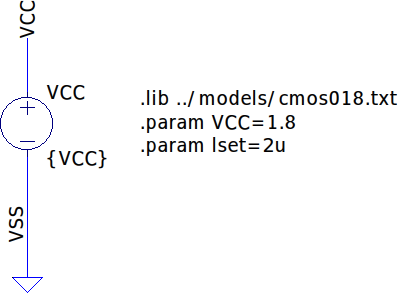
\includegraphics[scale=0.5]{spice0.png}
  \caption{Společná část SPICE kódu a napájecí zdroj.}
  \label{fig:spice0-png}
\end{figure}
 
\clearpage
\subsection{Ruční návrh}
Označení součástek v této kapitole odpovídá Obr.~\ref{fig:spice1.png}.

Nejprve zvolíme hodnotu kompenzační kapacity:
\[
    C_{C} = \num{0.3}\cdot C_{L} = \num{0.3}\cdot  \num{5e-12} = \qty{1.5}{pF}
\] 

Dále je potřeba stanovit minimální potřebné proudy v obvodu:
\begin{align*}
    GBW &= \frac{\frac{2\cdot I_{1} }{U_{OV1} }}{2\cdot \pi \cdot C_{C} } \\ 
    I_{1} &= U_{OV1}\cdot \pi \cdot C_{C} \cdot GBW \\ 
    I_{1} &= \num{0.2}\cdot \pi \cdot \num{1.5e-12} \cdot \num{10e6} \\ 
    I_{1} &= \qty{9.42}{\micro A}
\end{align*}

\begin{align*}
    SR_{int}  &= \frac{I_{p3}}{C_{C} } \\ 
    I_{p3} &= SR_{int}\cdot C_{C}  \\
    I_{p3} &= \num{5e6}\cdot \num{1.5e-12}  \\
    I_{p3} &= \qty{7.5}{\micro A}  \\
\end{align*}

    Aby bylo vyhověno všem parametrům a zachována jistá návrhová rezerva byl zvolen proud \(I_{p3} =\qty{20}{\micro A}\) a proudy \(I_{1}=I_{2}= \qty{10}{\micro A}  \).

    Ze stanovených proudů lze vypočítat rozměry tranzistorů:
    \begin{align*}
        \frac{W_{p3}}{L} &= \frac{2\cdot I_{p3}}{KP_{P}\cdot (U_{GS} -U_{TH})^2 } \\
        \frac{W_{p3}}{L} &= \frac{2\cdot \num{20e-6}}{\num{60e-6}\cdot \num{0.2}^2 } \\
        \frac{W_{p3}}{L} &= \num{16.67}
    \end{align*}
    Tedy \(W_{p3} = \qty{33.33}{\micro m}\). Proud touto větví se dále dělí na půl, tedy platí \(W_{p1,2} = W_{p3} /2 = \qty{16.67}{\micro m}\). 

    Ekvivalentní výpočet pro tranzistorů typu N:
    \begin{align*}
        \frac{W_{n1,2}}{L} &= \frac{2\cdot I_{n1,2}}{KP_{N}\cdot (U_{GS} -U_{TH})^2 } \\
        \frac{W_{n1,2}}{L} &= \frac{2\cdot \num{10e-6}}{\num{220e-6}\cdot \num{0.2}^2 } \\
        \frac{W_{n1,2}}{L} &= \num{2.27}
    \end{align*}
    Tedy \(W_{n1,2} = \qty{4.54}{\micro m}\).

    Z podmínky pro fázovou bezpěčnost alespoň \qty{60}{\degree} vyplývá pro druhý stupeň desetkrát větší proud než pro první stupeň. Tedy i rozměry tranzistorů ve výstupní větvi budou desetkrát větší, platí:
    \begin{align*}
        W_{p4} &= 10\cdot W_{p2} = \qty{166.7}{\micro m} \\
        W_{n3} &= 10\cdot W_{n2} = \qty{45.4}{\micro m} \\
    \end{align*}

    Pro poslední tranzistor \(M_{p5} \) zvolíme stejný proud (a tedy i rozměry) jako pro \(M_{p3} \), zbývá dopočíst hodnotu \(R_{1}\):
    \begin{align*}
        R_{1} &= \frac{U_{CC} - (U_{DSp5min} + U_{TH0p5})  }{I_{p5} } \\
        R_{1} &= \frac{\num{1.8} - (\num{0.2} + \num{0.43}) }{\num{20e-6} } \\
        R_{1} &= \qty{58.5}{k\ohm}
    \end{align*}

    

\subsubsection{Předpokládané hodnoty parametrů}
    Na základě zvolených hodnot proudů a rozměrů součástek je potřeba znovu přepočítat některé parametry:
    \begin{align*}
        GBW &= \frac{\frac{2\cdot I_{1} }{U_{OV1} }}{2\cdot \pi \cdot C_{C} } \\ 
        GBW &= \frac{\frac{2\cdot \num{10e-6} }{\num{0.2} }}{2\cdot \pi \cdot \num{1.5e-12} } \\ 
        GBW &= \qty{10.61}{MHz}
    \end{align*}

    \begin{align*}
        SR_{int}  &= \frac{I_{p3}}{C_{C} } \\ 
        SR_{int}  &= \frac{\num{20e-6}}{\num{1.5e-12}} \\ 
        SR_{int}  &= \qty{13.33}{V \per\micro s}
    \end{align*}

    Odhadovaná spotřeba zařízení:
    \begin{align*}
        P&=U_{CC}\cdot (I_{p5} +I_{p3} +I_{p4} ) \\
        P&=\num{1.8}\cdot (\num{20e-6} +\num{20e-6} +\num{100e-6} ) \\
        P&=\qty{252.00}{\micro W} \\
    \end{align*}

    Vstupní rozsah souhlasného napětí:
    \begin{align*}
        U_{ICMRmin} &= U_{TH,n}-U_{TH,p} +U_{OV3} \\ 
        U_{ICMRmin} &= \num{387.106e-3}-\num{443.3e-3} +\num{0.2} \\ 
        U_{ICMRmin} &= \qty{143,8}{mV}
    \end{align*}

    \begin{align*}
        U_{ICMRmax} &= U_{TH,p} + U_{OV1} + U_{OV5}  \\ 
        U_{ICMRmax} &= \num{443.3e-3} +\num{0.2}+\num{0.2} \\ 
        U_{ICMRmax} &= \qty{843.3}{mV}
    \end{align*}

    Výstupní napětový rozsah:
    \begin{align*}
        OVS &= U_{CC} -U_{OV7} -U_{OV6} \\ 
        OVS &= \num{1.8} -\num{0.2} -\num{0.2} \\
        OVS &= \qty{1.4}{V}
    \end{align*}

    Zesílení:
    \begin{align*}
    A_{U0} &= g_{m 1} \cdot\left(r_{D S 2} \| r_{D S 4}\right) \cdot g_{m 6} \cdot\left(r_{D S 6} \| r_{D S 7}\right) \\
    A_{U0} &= \frac{2\cdot I_{1}}{U_{OV1}} 
        \cdot\left(\frac{\frac{1}{\lambda_2 I_2} \cdot \frac{1}{\lambda_4 I_4}}{\frac{1}{\lambda_2 I_2}+\frac{1}{\lambda_4 I_4}}\right) \cdot \frac{2\cdot I_{6} }{U_{OV6} } 
        \cdot\left(\frac{\frac{1}{\lambda_6 I_6} \cdot \frac{1}{\lambda_7 I_7}}{\frac{1}{\lambda_6 I_6}+\frac{1}{\lambda_7 I_7}}\right) \\
    A_{U0} &= \frac{2\cdot \num{10e-6}}{\num{0.2}} 
        \cdot\left(\frac{\frac{1}{\num{0.08}\cdot  \num{10e-6}} \cdot \frac{1}{\num{0.04}\cdot  \num{10e-6}}}{\frac{1}{\num{0.08}\cdot  \num{10e-6}}+\frac{1}{\num{0.04}\cdot  \num{10e-6}}}\right) \cdot \frac{2\cdot \num{100e-6} }{\num{0.2} } 
        \cdot\left(\frac{\frac{1}{\num{0.04}\cdot  \num{100e-6}} \cdot \frac{1}{\num{0.08}\cdot  \num{100e-6}}}{\frac{1}{\num{0.04} \cdot \num{100e-6}}+\frac{1}{\num{0.08}\cdot  \num{100e-6}}}\right) \\
        A_{U0} &= \num{6944.44} = \qty{76.83}{dB}
    \end{align*}





\subsubsection{Zapojení na tranzistorové úrovni}
    \begin{figure}[h!]
        \centering
        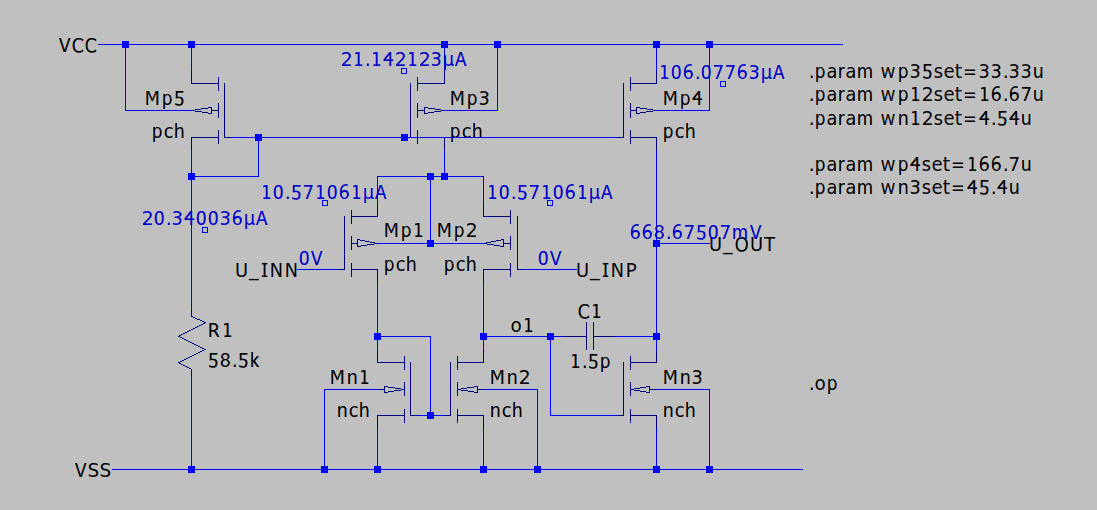
\includegraphics[scale=0.5]{spice1.png}
        \caption{Vnitřní zapojení OTA zesilovače.}
        \label{fig:spice1.png}
    \end{figure}
    
    Z analýzy .OP lze vypočítat spotřebu zapojení:
    \begin{align*}
        P&=U_{CC}\cdot (I_{p5} +I_{p3} +I_{p4} ) \\
        P&=\num{1.8}\cdot (\num{20.34e-6} +\num{21.142e-6} +\num{106.07e-6} ) \\
        P&=\qty{265.59}{\micro W} \\
    \end{align*}


\clearpage
\subsection{Zapojení pro .OP analýzu}
\begin{figure}[h!]
    \centering
    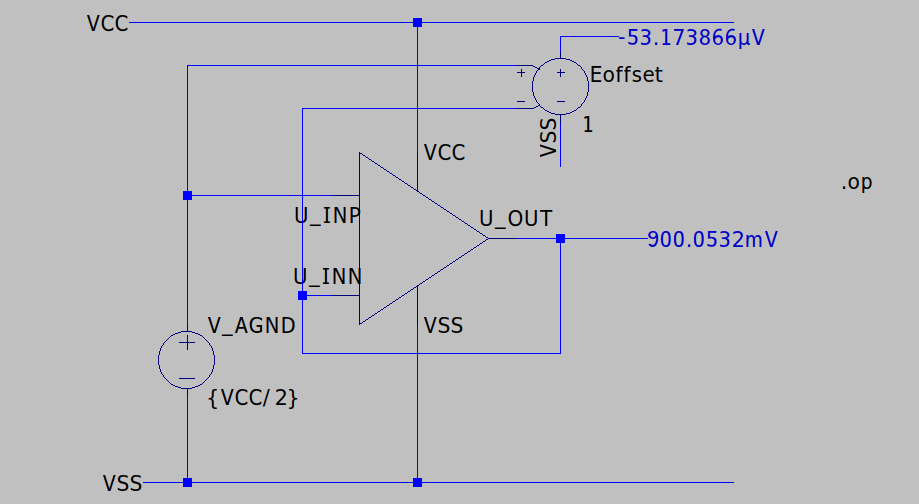
\includegraphics[scale=0.5]{spiceOP.png}
    \caption{Zapojení pro .OP analýzu.}
    \label{fig:spiceOP.png}
\end{figure}

\clearpage
\subsection{Analýza .AC}
Natevení filtru typu DP pro \(f_{m} =  \qty{1}{Hz}\) :
\begin{align*}
    \tau &= \frac{1}{\omega} \\
    R\cdot C &= \frac{1}{2\cdot \pi \cdot f_{RC} } \\
    R\cdot C &= \frac{1}{2\cdot \pi \cdot 1 } \\
    R\cdot C &= \num{0.16} \\
\end{align*}

Pokud zvolíme \(R=\qty{1}{M\ohm}\), pro kondenzátor vychází \(C=\num{0.16}/1000 = \qty{160}{nF}\) 

\begin{figure}[h!]
    \centering
    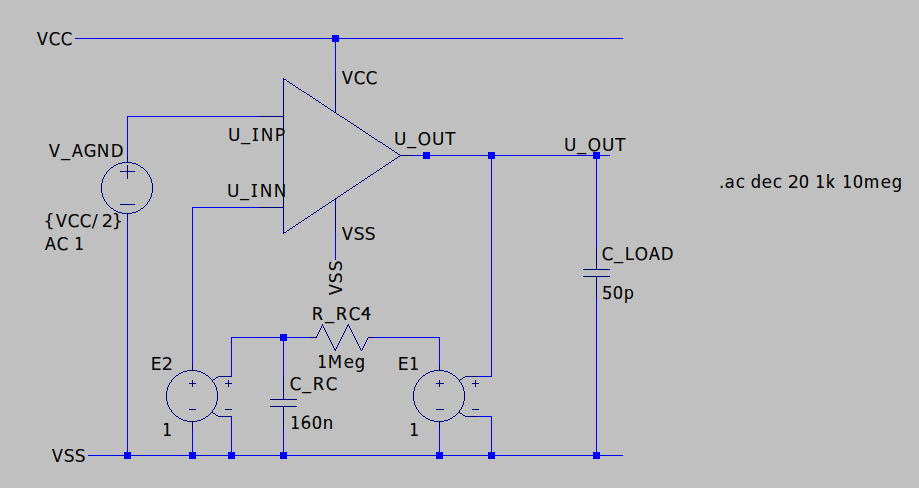
\includegraphics[scale=0.5]{spiceAC.png}
    \caption{Zapojení pro .AC analýzu.}
    \label{fig:spice1.png}
\end{figure}

\begin{figure}[h!]
    \centering
    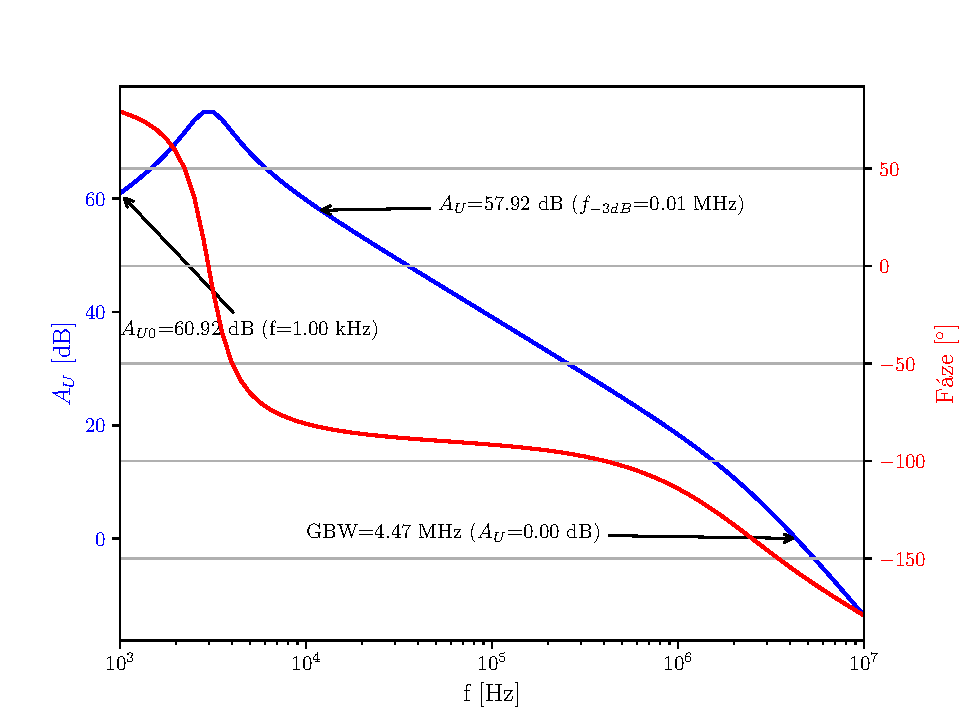
\includegraphics[]{AC.pdf}
    \caption{Výsledky .AC analýzy.}
    \label{fig:spice1.png}
\end{figure}




\clearpage
\subsection{Analýza .DC}
\begin{figure}[h!]
    \centering
    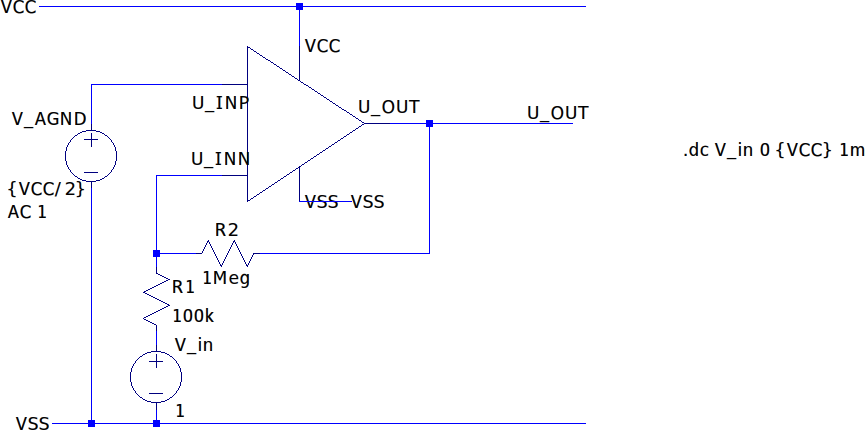
\includegraphics[scale=0.5]{spiceOVS.png}
    \caption{Zapojení pro .DC analýzu OVS.}
    \label{fig:spiceOVS.png}
\end{figure}

\begin{figure}[h!]
    \centering
    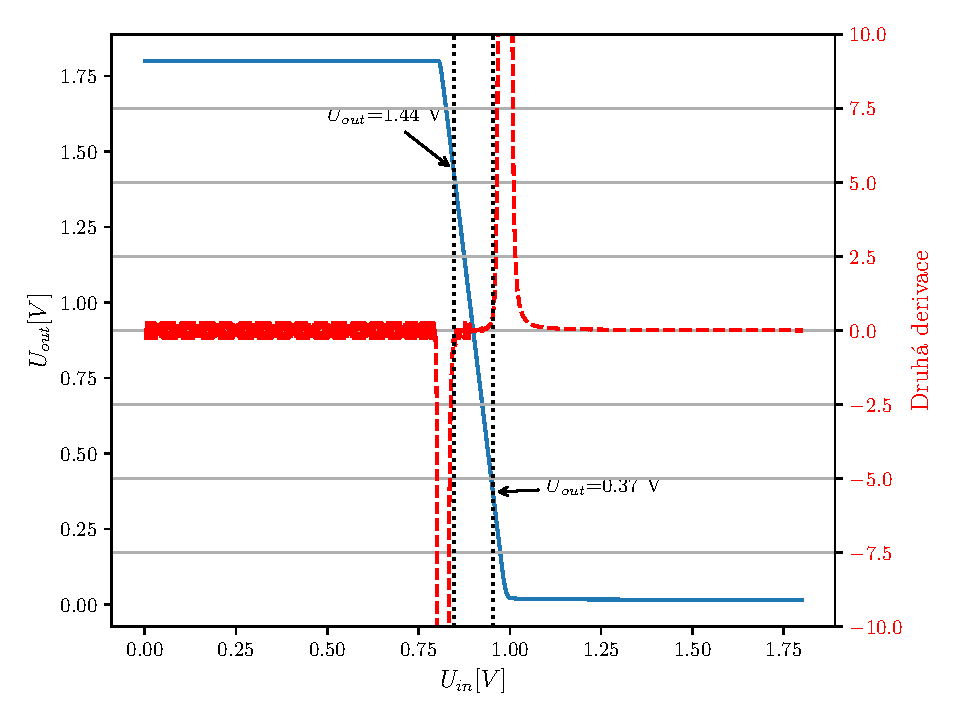
\includegraphics[]{OVS.pdf}
    \caption{Výsledky .DC analýzy pro měření OVS.}
    \label{fig:OVS.pdf}
\end{figure}

\begin{figure}[h!]
    \centering
    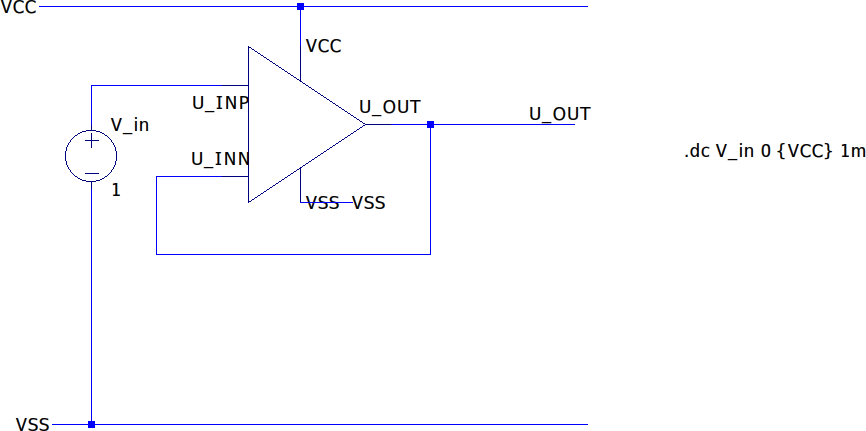
\includegraphics[scale=0.5]{spiceICMR.png}
    \caption{Zapojení pro .DC analýzu ICMR.}
    \label{fig:spiceICMR.png}
\end{figure}

\begin{figure}[h!]
    \centering
    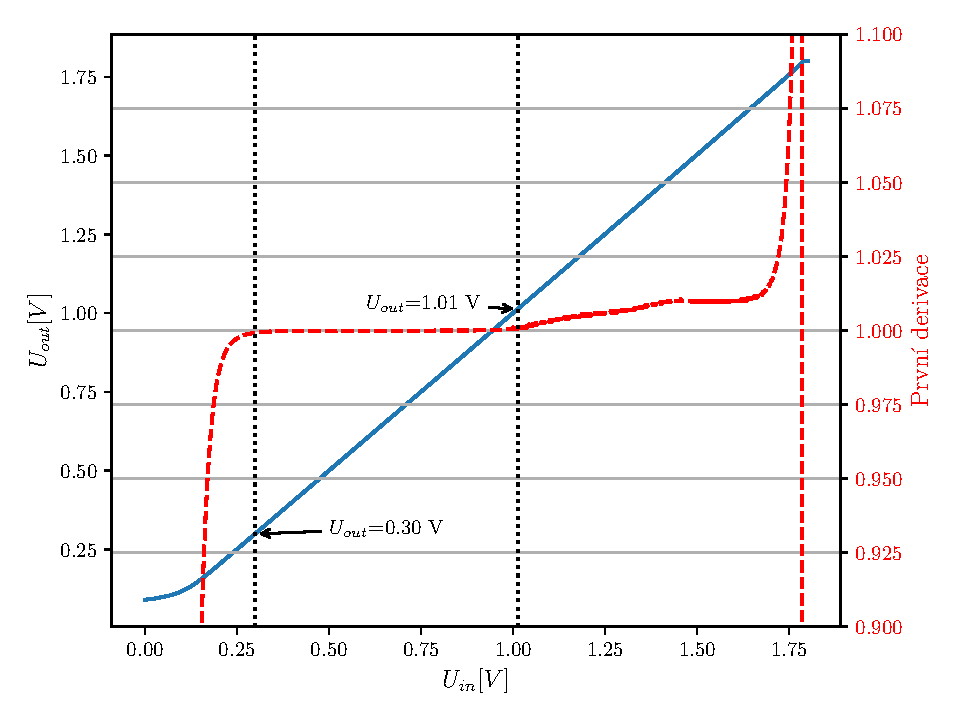
\includegraphics[]{ICMR.pdf}
    \caption{Výsledky .DC analýzy pro měření ICMR.}
    \label{fig:OVS.pdf}
\end{figure}




\clearpage
\subsection{Analýza .TRAN}
\begin{figure}[h!]
    \centering
    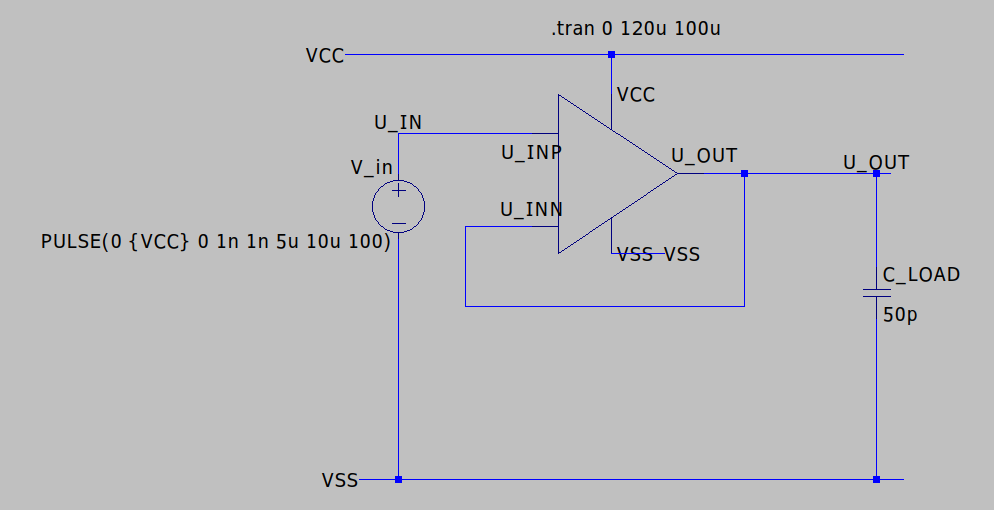
\includegraphics[scale=0.5]{spiceTRAN.png}
    \caption{Zapojení pro .TRAN analýzu.}
    \label{fig:spice1.png}
\end{figure}

\begin{figure}[h!]
    \centering
    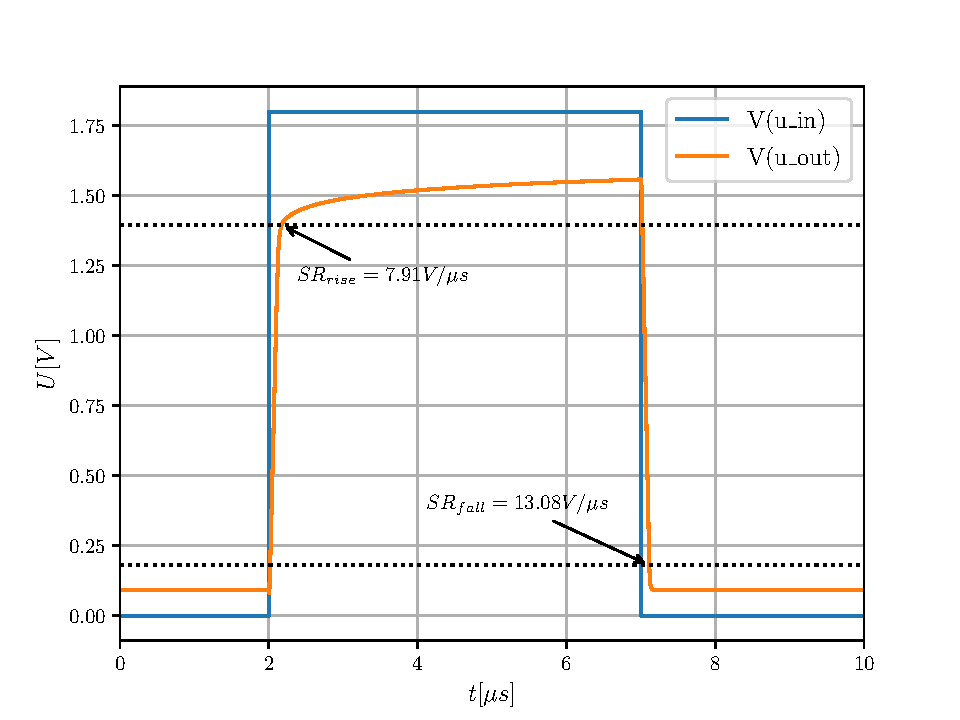
\includegraphics[]{TRAN.pdf}
    \caption{Výsledky .TRAN analýzy pro měření SR.}
    \label{fig:OVS.pdf}
\end{figure}




\clearpage
\section{Závěr}


\end{document}
